%%%%%%%%%%%%%%%%%%%%%%%%%%%%%%%%%%%%%%%%%
% Programming/Coding Assignment
% LaTeX Template
%
% This template has been downloaded from:
% http://www.latextemplates.com
%
% Original author:
% Ted Pavlic (http://www.tedpavlic.com)
%
% Note:
% The \lipsum[#] commands throughout this template generate dummy text
% to fill the template out. These commands should all be removed when 
% writing assignment content.
%
% This template uses a Perl script as an example snippet of code, most other
% languages are also usable. Configure them in the "CODE INCLUSION 
% CONFIGURATION" section.
%
%%%%%%%%%%%%%%%%%%%%%%%%%%%%%%%%%%%%%%%%%

%----------------------------------------------------------------------------------------
%	PACKAGES AND OTHER DOCUMENT CONFIGURATIONS
%----------------------------------------------------------------------------------------

\documentclass{article}

\usepackage{fancyhdr} % Required for custom headers
\usepackage{lastpage} % Required to determine the last page for the footer
\usepackage{extramarks} % Required for headers and footers
\usepackage[usenames,dvipsnames]{color} % Required for custom colors
\usepackage{graphicx} % Required to insert images
\usepackage{listings} % Required for insertion of code
\usepackage{courier} % Required for the courier font
\usepackage{lipsum} % Used for inserting dummy 'Lorem ipsum' text into the template
\usepackage{setspace}
\usepackage{color}
\usepackage{comment}
\usepackage{caption}

\usepackage{hyperref}
\usepackage{natbib}
\usepackage{underscore}
\usepackage{subfigure}
\usepackage{fixltx2e}

\hypersetup{
    colorlinks=true,
    linkcolor=blue,
    filecolor=magenta,      
    urlcolor=cyan,
    breaklinks=true
}

%\usepackage[]{algorithm2e}
\usepackage{pdfpages}




%For python inclusion (http://widerin.org/blog/syntax-highlighting-for-python-scripts-in-latex-documents)
\definecolor{Code}{rgb}{0,0,0}
\definecolor{Decorators}{rgb}{0.5,0.5,0.5}
\definecolor{Numbers}{rgb}{0.5,0,0}
\definecolor{MatchingBrackets}{rgb}{0.25,0.5,0.5}
\definecolor{Keywords}{rgb}{0,0,1}
\definecolor{self}{rgb}{0,0,0}
\definecolor{Strings}{rgb}{0,0.63,0}
\definecolor{Comments}{rgb}{0,0.63,1}
\definecolor{Backquotes}{rgb}{0,0,0}
\definecolor{Classname}{rgb}{0,0,0}
\definecolor{FunctionName}{rgb}{0,0,0}
\definecolor{Operators}{rgb}{0,0,0}
\definecolor{Background}{rgb}{0.98,0.98,0.98}

% Margins
\topmargin=-0.45in
\evensidemargin=0in
\oddsidemargin=0in
\textwidth=6.5in
\textheight=9.0in
\headsep=0.25in

\linespread{1.1} % Line spacing

% Set up the header and footer
\pagestyle{fancy}
\lhead{\hmwkAuthorName} % Top left header
%\chead{\hmwkClass\ (\hmwkClassInstructor\ \hmwkClassTime): \hmwkTitle} % Top center head
\chead{\hmwkClass\ (\hmwkClassInstructor): \hmwkTitle} % Top center head
\rhead{\firstxmark} % Top right header
\lfoot{\lastxmark} % Bottom left footer
\cfoot{} % Bottom center footer
\rfoot{Page\ \thepage\ of\ \protect\pageref{LastPage}} % Bottom right footer
\renewcommand\headrulewidth{0.4pt} % Size of the header rule
\renewcommand\footrulewidth{0.4pt} % Size of the footer rule

\setlength\parindent{0pt} % Removes all indentation from paragraphs

%----------------------------------------------------------------------------------------
%	CODE INCLUSION CONFIGURATION
%----------------------------------------------------------------------------------------

\definecolor{MyDarkGreen}{rgb}{0.0,0.4,0.0} % This is the color used for comments
\lstloadlanguages{Perl} % Load Perl syntax for listings, for a list of other languages supported see: ftp://ftp.tex.ac.uk/tex-archive/macros/latex/contrib/listings/listings.pdf
\lstset{language=Perl, % Use Perl in this example
        frame=single, % Single frame around code
        basicstyle=\small\ttfamily, % Use small true type font
        keywordstyle=[1]\color{Blue}\bf, % Perl functions bold and blue
        keywordstyle=[2]\color{Purple}, % Perl function arguments purple
        keywordstyle=[3]\color{Blue}\underbar, % Custom functions underlined and blue
        identifierstyle=, % Nothing special about identifiers                                         
        commentstyle=\usefont{T1}{pcr}{m}{sl}\color{MyDarkGreen}\small, % Comments small dark green courier font
        stringstyle=\color{Purple}, % Strings are purple
        showstringspaces=false, % Don't put marks in string spaces
        tabsize=5, % 5 spaces per tab
        %
        % Put standard Perl functions not included in the default language here
        morekeywords={rand},
        %
        % Put Perl function parameters here
        morekeywords=[2]{on, off, interp},
        %
        % Put user defined functions here
        morekeywords=[3]{test},
       	%
        morecomment=[l][\color{Blue}]{...}, % Line continuation (...) like blue comment
        numbers=left, % Line numbers on left
        firstnumber=1, % Line numbers start with line 1
        numberstyle=\tiny\color{Blue}, % Line numbers are blue and small
        stepnumber=5 % Line numbers go in steps of 5
}

% Creates a new command to include a perl script, the first parameter is the filename of the script (without .pl), the second parameter is the caption
\newcommand{\perlscript}[2]{
\begin{itemize}
\item[]\lstinputlisting[caption=#2,label=#1]{#1.pl}
\end{itemize}
}


%----------------------------------------------------------------------------------------
%	DOCUMENT STRUCTURE COMMANDS
%	Skip this unless you know what you're doing
%----------------------------------------------------------------------------------------

% Header and footer for when a page split occurs within a problem environment
\newcommand{\enterProblemHeader}[1]{
\nobreak\extramarks{#1}{#1 continued on next page\ldots}\nobreak
\nobreak\extramarks{#1 (continued)}{#1 continued on next page\ldots}\nobreak
}

% Header and footer for when a page split occurs between problem environments
\newcommand{\exitProblemHeader}[1]{
\nobreak\extramarks{#1 (continued)}{#1 continued on next page\ldots}\nobreak
\nobreak\extramarks{#1}{}\nobreak
}

\setcounter{secnumdepth}{0} % Removes default section numbers
\newcounter{homeworkProblemCounter} % Creates a counter to keep track of the number of problems

\newcommand{\homeworkProblemName}{}
\newenvironment{homeworkProblem}[1][Problem \arabic{homeworkProblemCounter}]{ % Makes a new environment called homeworkProblem which takes 1 argument (custom name) but the default is "Problem #"
\stepcounter{homeworkProblemCounter} % Increase counter for number of problems
\renewcommand{\homeworkProblemName}{#1} % Assign \homeworkProblemName the name of the problem
\section{\homeworkProblemName} % Make a section in the document with the custom problem count
\enterProblemHeader{\homeworkProblemName} % Header and footer within the environment
}{
\exitProblemHeader{\homeworkProblemName} % Header and footer after the environment
}

\newcommand{\problemAnswer}[1]{ % Defines the problem answer command with the content as the only argument
\noindent\framebox[\columnwidth][c]{\begin{minipage}{0.98\columnwidth}#1\end{minipage}} % Makes the box around the problem answer and puts the content inside
}

\newcommand{\homeworkSectionName}{}
\newenvironment{homeworkSection}[1]{ % New environment for sections within homework problems, takes 1 argument - the name of the section
\renewcommand{\homeworkSectionName}{#1} % Assign \homeworkSectionName to the name of the section from the environment argument
\subsection{\homeworkSectionName} % Make a subsection with the custom name of the subsection
\enterProblemHeader{\homeworkProblemName\ [\homeworkSectionName]} % Header and footer within the environment
}{
\enterProblemHeader{\homeworkProblemName} % Header and footer after the environment
}

%----------------------------------------------------------------------------------------
%	NAME AND CLASS SECTION
%----------------------------------------------------------------------------------------
%#MOD
\newcommand{\hmwkTitle}{Assignment\ \#1 } % Assignment title
%\newcommand{\hmwkDueDate}{Monday,\ January\ 1,\ 2012} % Due date
\newcommand{\hmwkClass}{Web Science} % Course/class
%\newcommand{\hmwkClassTime}{10:30am} % Class/lecture time
\newcommand{\hmwkClassInstructor}{Alexander Nwala} % Teacher/lecturer
\newcommand{\hmwkAuthorName}{Mohd. Nauman Siddique} % Your name

%----------------------------------------------------------------------------------------
%	TITLE PAGE
%----------------------------------------------------------------------------------------

\title{
\vspace{2in}
\textmd{\textbf{\hmwkClass:\ \hmwkTitle}}\\
%\normalsize\vspace{0.1in}\small{Due\ on\ \hmwkDueDate}\\
%\vspace{0.1in}\large{\textit{\hmwkClassInstructor\ \hmwkClassTime}}
\vspace{0.1in}\large{\textit{\hmwkClassInstructor}}
\vspace{3in}
}

\author{\textbf{\hmwkAuthorName}}
%#MOD
\date{Thursday, January 31, 2019} % Insert date here if you want it to appear below your name

%----------------------------------------------------------------------------------------

\begin{document}

\maketitle



%----------------------------------------------------------------------------------------
%	TABLE OF CONTENTS
%----------------------------------------------------------------------------------------

%\setcounter{tocdepth}{1} % Uncomment this line if you don't want subsections listed in the ToC

\newpage
\tableofcontents
\newpage

%----------------------------------------------------------------------------------------
%	PROBLEM 1
%----------------------------------------------------------------------------------------

% To have just one problem per page, simply put a \clearpage after each problem

\begin{homeworkProblem}
Demonstrate that you know how to use "curl" well enough to correctly POST data to a form.  Show that the HTML response that
is returned is "correct".  That is, the server should take the arguments you POSTed and build a response accordingly.  Save the
HTML response to a file and then view that file in a browser and take a screen shot.

Feel free to use my simple server for sending POST requests:
\url{ http://www.cs.odu.edu/~anwala/files/temp/namesEcho.php}
The server needs you to POST data for "fname" and "lname" fields.

%\problemAnswer
%{
    \begin{verbatim}\end{verbatim}
    \textbf{SOLUTION}\\

The solution to the problem is as below:
\begin{enumerate}
 \item \textbf{Curl Command}: curl \cite{Curl} command to send parameters to a server and save its response to a html file is provided below.
\begin{lstlisting}[language=bash, breaklines=true]
$ curl -d "fname=nauman&lname=siddique"  -X  POST http://www.cs.odu.edu/~anwala/files/temp/namesEcho.php > response.html
\end{lstlisting}
\item \textbf{Curl Redirect}: The command redirects with 301 and its output can be seen in figure \ref{TerminalRedirect} and figure \ref{BrowserlRedirect}.
\begin{figure}[ht]
  \centering
  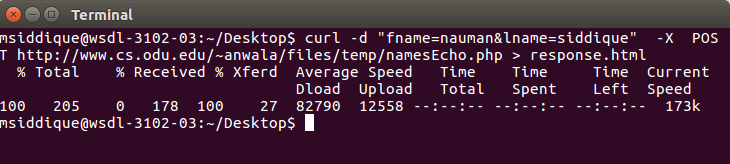
\includegraphics[width=0.9\textwidth]{Redirect.png}
  \caption{Terminal screenshot for curl redirect on \url{ http://www.cs.odu.edu/~anwala/files/temp/namesEcho.php}}
  \label{TerminalRedirect}
\end{figure}
\begin{figure}[ht]
  \centering
  
\includegraphics[width=0.9\textwidth]{RedirectScreenshot.png}
  \caption{Browser screenshot for curl redirect on \url{ http://www.cs.odu.edu/~anwala/files/temp/namesEcho.php}}
  \label{BrowserlRedirect}
\end{figure}
\item \textbf{Curl https}: The command reolves with a status code of 200 and it can be seen in figure \ref{TerminalHttps} and figure \ref{BrowserHttps}.
\begin{figure}[ht]
  \centering
  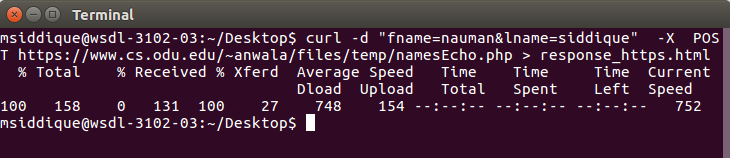
\includegraphics[width=0.9\textwidth]{Curlhttps.png}
  \caption{Terminal screenshot for curl on \url{ https://www.cs.odu.edu/~anwala/files/temp/namesEcho.php}}
  \label{TerminalHttps}
\end{figure}
\begin{figure}[ht]
  \centering
  
\includegraphics[width=0.9\textwidth]{ResponseScreenshot.PNG}
  \caption{Browser screenshot for curl on \url{ https://www.cs.odu.edu/~anwala/files/temp/namesEcho.php}}
  \label{BrowserHttps}
\end{figure}
\end{enumerate}
  
%}

\end{homeworkProblem}

%----------------------------------------------------------------------------------------
%   PROBLEM 2
%----------------------------------------------------------------------------------------

\begin{homeworkProblem}

 Write a Python program that:
\begin{enumerate}
  \item takes as a command line argument a web page
  \item extracts all the links from the page 
  \item lists all the links that result in PDF files, and prints out the bytes for each of the links.  (note: be sure to follow
     all the redirects until the link terminates with a "200 OK".)
  \item show that the program works on 3 different URIs, one of which      needs to be: 
     \url{http://www.cs.odu.edu/~mln/teaching/cs532-s17/test/pdfs.html}
\end{enumerate}

%\problemAnswer
%{
    \begin{verbatim}\end{verbatim}
    \textbf{SOLUTION}\\

\lstinputlisting[language=Python, breaklines=true]{LinkExtractor.py}
  The solution for this problem is outlined by the following steps:\\ \\
 \textbf{Assumption}: For the purpose of this assignment, I have restricted extracting links from web pages to one hop from the argument url.\\
\textbf{Command Line Argument}: The code accepts command line argments. In case of no argument supplied the default argument is \url{https://www.cs.odu.edu/~mln/teaching/cs532-s17/test/pdfs.html}.\\
\textbf{Extracting Links}: For extracting links, Beautiful Soup library of python has been used to check for all the "a" tags with href attribute.  \\
\textbf{Finding PDFs}: For finding pdf links, we have relied on the content-type in the respponse header which should be "application-pdf".\\
\textbf{Following Redirects}: In case of redirects, the redirect links are added to the frontier which runs till the frontier runs itself empty.\\
\textbf{Urls used for testing the code}: 
\begin{verbatim}
1. https://www.cs.odu.edu/~mln/teaching/cs532-s17/test/pdfs.html
2. https://odu.edu/compsci
3. https://www.cs.odu.edu/~mln/
\end{verbatim} 
\textbf{Show Results}:  PDF links extracted from the three urls are shown below.
\lstinputlisting[language={}, breaklines=true]{PDFLinks1.txt}
\lstinputlisting[language={}, breaklines=true]{PDFLinks2.txt}
\lstinputlisting[language={}, breaklines=true]{PDFLinks3.txt}
   %}

\end{homeworkProblem}

%----------------------------------------------------------------------------------------
%   PROBLEM 3
%----------------------------------------------------------------------------------------

\begin{homeworkProblem}

Consider the "bow-tie" graph in the Broder et al. paper:
   \url{ http://snap.stanford.edu/class/cs224w-readings/broder00bowtie.pdf}

    Many have found this link useful: \url{https://www.harding.edu/fmccown/classes/archive/comp475-s13/web-structure-homework.pdf}
    Now consider the following graph:

    $A --> B$\\
    $B --> C$\\
    $C --> D$\\
    $C --> A$\\
    $C --> G$\\
    $E --> F$\\
    $G --> C$\\
   $ G --> H$\\
    $I --> H$\\
    $I --> K$\\
    $L --> D$\\
    $M --> A$\\
    $M --> N$\\
    $N --> D$\\
    $O --> A$\\
   $ P --> G $\\
    
    For the above graph, give the values for:

    IN: \\
    SCC: \\
    OUT: \\
    Tendrils:\\ 
    Tubes: \\
    Disconnected:\\

%\problemAnswer
%{
    \begin{verbatim}\end{verbatim}
    \textbf{SOLUTION}\\
The graph for the bow-tie structure is converted as shown below and is being used as input to the python code.
\begin{figure}[ht]
  \centering
  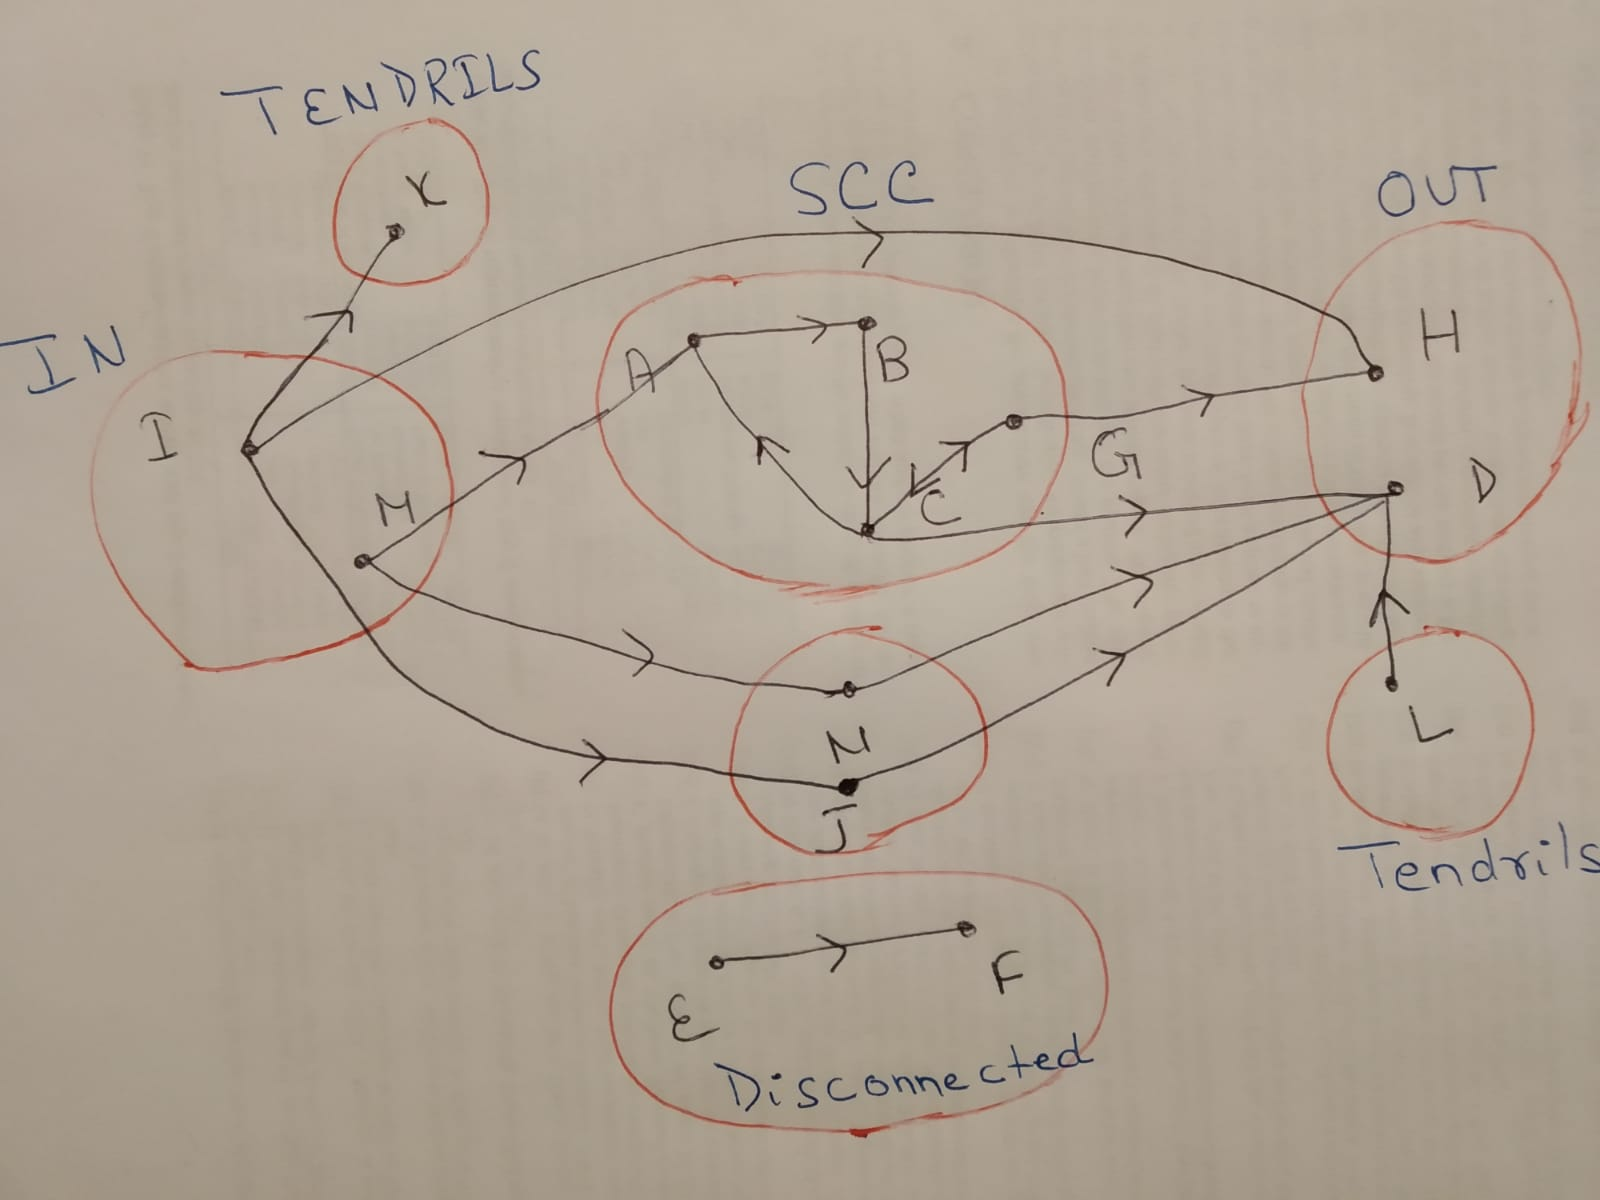
\includegraphics[width=0.9\textwidth, keepaspectratio]{Graph.jpg}
  \caption{Graph for bow-tie}
  \label{Graph}
\end{figure}
\lstinputlisting[language={}, breaklines=true]{GraphInput.txt}
\lstinputlisting[language=Python, breaklines=true]{BowTie.py}
The graph has been shown in figure \ref{Graph} which shows all the different categories of points which have been explained below.
The output is calculated with below mentioned categories of points:
\begin{enumerate}
\item \textbf{SCC}: points which have both incoming and outgoing edges. They are connected to points within IN, OUT and SCC.
\item \textbf{IN}: points which have only outgoing edges and are connected to SCC.
\item \textbf{OUT}: points which have only incoming edges and are connected to SCC.
\item \textbf{Tendrils}: points which have either incoming or outgoing edges connected to IN or OUT.
\item \textbf{Tube}: points which have inlinks from IN and outlinks to OUT.
\item \textbf{Disconnected}: points which are not connected to IN, OUT and SCC.
\end{enumerate}
The output to the program listing all the points is shown in figure \ref{BowTieOutput} and are also listed below.
\begin{enumerate}
\item \textbf{SCC}: a, b, c, g
\item \textbf{IN}: i, m
\item \textbf{OUT}: d, h
\item \textbf{Tendrils}: k, l
\item \textbf{Tube}: j, n
\item \textbf{Disconnected}: e, f
\end{enumerate}
\begin{figure}[ht]
  \centering
  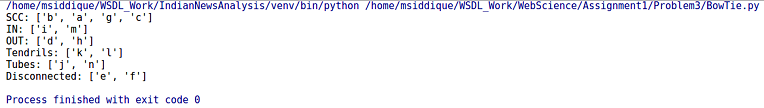
\includegraphics[width=0.9\textwidth, height = 4cm, keepaspectratio]{BowTie.PNG}
  \caption{Output of BowTie Program}
  \label{BowTieOutput}
\end{figure}
\end{homeworkProblem}
\bibliographystyle{plain}
\bibliography{A2bibFile}

\end{document}
    


   

    

    

    
   
